\documentclass{article}

\usepackage{graphicx}

\title{CSE434 Project Report}
\author{Ben Chavet, James Dicke}
\date{\today}

\begin{document}
  \maketitle

  \section{Summary}

  Ternary Content-Addressable Memory, or CAMs, are a specialized variant of memory that contains 
  additional functionality beyond that of standard computer memory.  CAMs are designed primarily 
  for the purpose of fast searching applications, and are designed so that a search operation 
  completes in a single clock cycle.  The two most common uses of CAM architecture are
  hardware-based packet forwarding and packet classification present in routers. \cite{campaper}

  CAMs, with their increased functionality, are not used as standard computer memory due to the 
  increased amount of circuitry.  Each memory location in the CAM must contain a memory address, 
  the memory contents, as well as logic to compare the input address to the address stored in the 
  memory location.  By comparison, each memory location in standard memory only contains the 
  memory contents.

  Ternary CAMs add additional functionality to a standard CAM in the ability to specify unknowns
  when searching for an address.  More information is contained in the next section.

  \section{Background}

  Standard memory uses a static address space to access its contents.  In
  order to access a value, you must know its address.  In contrast, a CAM uses a
  key/value pair, much like how an associative array works in software.  Data
  in a CAM is accessed by its key instead of by its address. In addition, a 
  ternary CAM allows the use of ``don't care'' values when specifying the key.
  This adds flexibility in the search functionality of a CAM. \cite{wikipedia}

  \section{Operations}

  The basic functions of our CAM are: read, write, delete, and reset.
  Except for reset, all of the operations rely on searching the
  CAM for keys that match the key/mask input pair.  This input generates a
  search key such that the bits of the input key that correspond to the bits
  of the mask that are set to ``0'' are used literally.  The bits that
  correspond to the bits of the mask that are set to ``1'' are considered to
  be ``don't cares.''

  The search for a match to the key/mask input pair is very fast.  Every
  slice in the CAM checks whether it matches in parallel, so all matches
  are found at the same time.  At that point, the logic that chooses the
  first match kicks in.  By arbitrarily choosing the first match in the
  CAM, (instead of, say, the ``best'' match), we are able to push the output
  through the chip using the shortest possible path.

  \subsection{Read}

  Read uses the match function described above to send the value corresponding
  to the first matched key to the CAM's output.  If no match is found, the
  {\it notFound} output is asserted, and all of the output bits are set to
  zero.

  \subsection{Write}

  Write is easily the most complicated function of the CAM.  It first checks for
  a match from the key/mask inputs.  If one (or more) is found, the value
  corresponding with that match is overwritten with the input data.  However,
  if no match is found, the input data word is stored at an unused storage
  space.  If there are no unused spaces, the value is not written, and the
  {\it full} output is asserted.

  Due to the complexity of the write operation, it is also slow.  This is
  minimized by making the search function as fast as possible.

  \subsection{Delete}

  Delete works in the same manner as Write.  It deletes the key and value
  corresponding to the match.  If no match is found, nothing is done.

  \subsection{Reset}

  Reset is as simple as it sounds.  When the {\it reset} input is asserted, the
  entire contents of the CAM are deleted, resulting in an empty CAM.

  A reset must be the first operation performed when initializing the chip for use.

  \section{Additional Features}

  \subsection*{Low Power Consumption}

  Low power consumption on our CAM is mostly a side effect of the modular design
  we used.  By default every connection from the data storage to the output
  line is disabled, and is only enabled when it is being read.  This means that
  at any given time, only one data slice is ``active'' and using power.

  In addition, the matching logic works in a similar fashion.  Each bit of the
  stored key must match the input key/mask pair in order to match.  So, if any
  bit does not match, none of the remaining bits are checked, thus saving power.

  \subsection*{Chaining}

  Another feature of our CAM is the ability to chain multiple CAMs in series,
  allowing them to act as one continuous CAM unit.  All inputs and outputs necessary to make this possible are specifically included.

  Each CAM unit shares the same key, mask, input word, {\it write}, {\it delete}, and
  {\it reset} lines.  Each CAM's {\it notFoundPrev} is connected to the previous CAM's {\it notFound},
  connecting the first CAM's {\it notfoundPrev} to Vdd.  {\it NotFound} on the last CAM, if asserted, 
  indicates that there were no matches in any of the CAMs in the chain.

  When a CAM has searched all its addresses and fails to match the input key/mask pair, it asserts its own {\it notFound} output.  Each CAM in the chain
  performs this step in parallel.  If multiple CAMs do not assert the {\it notFound} output signifying that there are multiple matches, the {\it notFound} output
  is used to signify all CAMs but the first to de-assert their {\it notFound} output.

  If the key/mask pair has been matched, the memory contents corresponding to the match 
  are then passed to the next CAM in the chain, and the correct memory contents are eventually propagated all the way to the last CAM in the chain as the final output.

  \section{Inputs and Outputs}

  \subsection*{Inputs}
  \begin{itemize}
  \item \textbf{8-bit key:}
  \item \textbf{8-bit mask:}
    Specifies which bits of the key are ``don't cares''.
  \item \textbf{16-bit input word:}
    The word to be written
  \item \textbf{write:}
    When asserted, the input key and input word are written to memory.  When
    not asserted, a read operation is performed based on the input key and
    mask.
  \item \textbf{delete:}
    When asserted, the first entry with a key that matches the input key/mask
    pair is cleared to make room for new input.
  \item \textbf{reset:}
    When asserted, the entire contents of the CAM are cleared.
  \item \textbf{notFoundPrev:}
    Used for chaining.  When asserted, signifies that a match has already
    been found in a previous CAM unit.
  \item \textbf{fullPrev:}
    Used for chaining.  When asserted, signifies that a previous CAM unit is full and that the current CAM unit should attempt to handle writes.
  \end{itemize}

  \subsection*{Outputs}
  \begin{itemize}
  \item \textbf{16-bit output word:}
  \item \textbf{full:}
    Asserted when all memory locations are in use.
  \item \textbf{notFound:}
    Asserted when no addresses in the CAM match the key/mask input pair.  This is used to differentiate between when
    a match is not found, and when the content of the address matching the key/mask input is actually 0x00.
  \end{itemize}

  \section{Slice Schematic}

  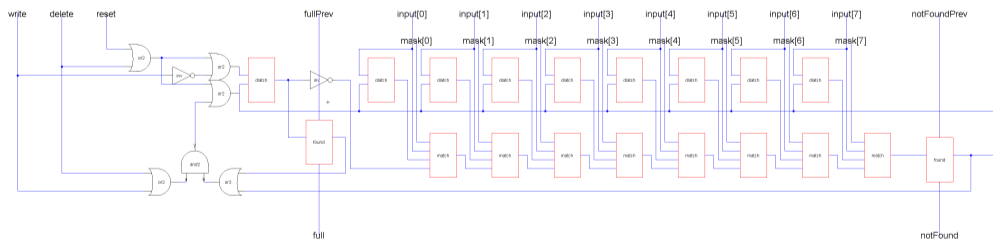
\includegraphics[height=30mm]{slice1-sch.png}
  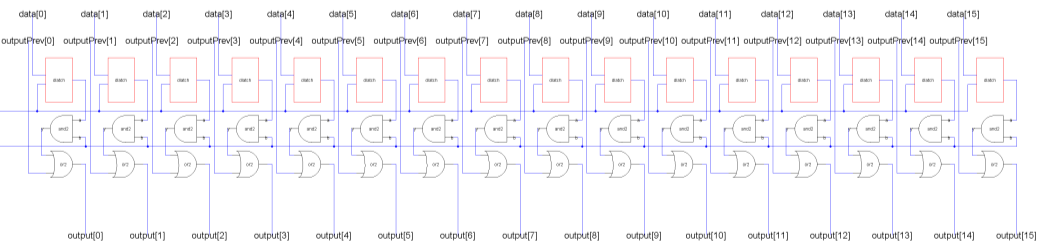
\includegraphics[height=30mm]{slice2-sch.png}

  \section{Leaf Cells}

  The leaf cells we chose to implement are XNOR2 and a D-Latch.  Each of these
  cells can be implemented using NAND gates, but by specifically designing them
  at the transistor level, we were able to significantly cut down the size
  that each of these cells use.  We chose these two cells because there are a
  large number of both of them in our design.  In addition, any decrease in propagation time from these cells would result in the maximum improvement in speed of memory reads.

  \subsection*{XNOR2}

  The NAND implementation of the XNOR2 gate used five NAND2 gates, requiring approximately 13,000 square lambda.  In each CAM unit, 128 XNOR2 gates were
  required, requiring a total of approximately 1,664,000 square lambda.  For this reason, a customized XNOR2 of decreased size was created, requiring only
  approximately 7,500 square lambda per gate, and reducing the total size for XNOR2s to less than one million square lambda.  In addition, the customized
  XNOR2 implementation was significantly faster.  The NAND implementation propagation delay required 350 ps from high to low output and 500 ps from low to high
  output, while the customized gate delays were 100 ps and 130 ps respectively.

  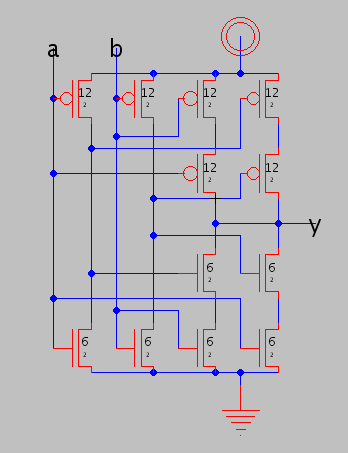
\includegraphics[height=60mm]{xnor-sch.png}
  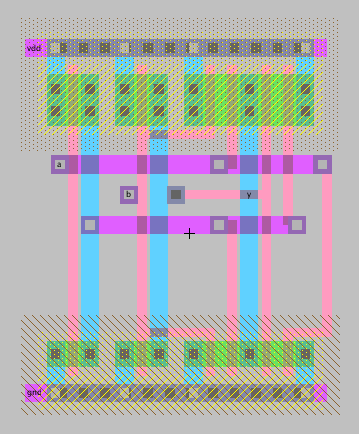
\includegraphics[height=60mm]{xnor-lay.png}

  \subsection*{D-Latch}

  The NAND implementation of the D latch used four NAND2 gates.  A customized D latch was also designed to reduce chip size.  Each CAM unit contained 
  272 latches, and as a result of the customized D latch, the total chip area dedicated to D latches was reduced from approximately 3.2 million square lambda 
  to 1.9 million square lambda.  The customized latch was also faster, decreasing the propagation delay through the latch from 2.3 ns to 300 ps, a considerable improvement.

  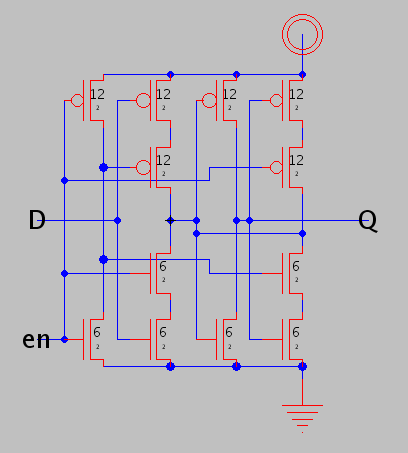
\includegraphics[height=60mm]{dlatch-sch.png}
  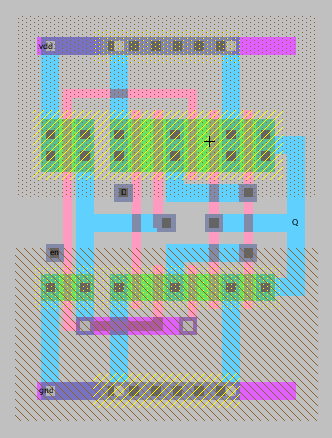
\includegraphics[height=60mm]{dlatch-lay.png}

  \section{Timing}
  The CAM, when tested at a system level, is able to successfully retrieve memory contents in approximately 13ns.
  This number was obtained by starting at 10ns and finding that the outputs were not valid.  Then, the same tests
  were run at 15ns, and the outputs were valid.  By trial and error, we found that the outputs are valid at
  13ns.

  Memory contents that are physically located at subsequent 
  memory locations will be retrieved more quickly.  In effect, a matching address contained in the first memory location will be slower than an address contained in the last memory location.
  This is an effect of the correct data having to propagate through all subsequent memory locations before reaching the final output.

  \begin{thebibliography}{1}
  \bibitem{dlatch1} http://tams-www.informatik.uni-hamburg.de/applets/cmos/cmosdemo.html
  \bibitem{dlatch2} http://tech-www.informatik.uni-hamburg.de/applets/hades/webdemos/05-switched/40-cmos/latch.html
  \bibitem{dlatch3} http://java.icmc.usp.br/dilvan/thesis.phd/result.html
  \bibitem{wikipedia} http://en.wikipedia.org/wiki/Content-addressable\_memory
  \bibitem{camintro} http://www.pagiamtzis.com/cam/camintro.html
  \bibitem{campaper} K. Pagiamtzis and A. Sheikholeslami, ``Content-addressable memory (CAM) circuits and architectures: A tutorial and survey,'' IEEE Journal of Solid-State Circuits, vol. 41, no. 3, pp. 712�727, March 2006. 
  \end{thebibliography}

\end{document}